% !TEX TS-program = pdflatexmk
\documentclass[11pt]{article}

\usepackage[margin=1in]{geometry}\headsep = 0.2 in
%\parskip = 0.2in
%\parindent = 0.0in

\usepackage{amsmath,amssymb,latexsym,graphicx,amsthm,enumerate}
\usepackage{palatino, url, multicol,tikz}
\newtheorem{theorem}{Theorem}
\newtheorem{corollary}[theorem]{Corollary}
\newtheorem{conjecture}[theorem]{Conjecture}
\newtheorem{lemma}[theorem]{Lemma}
\newtheorem{proposition}[theorem]{Proposition}
\newtheorem{definition}[theorem]{Definition}
\newtheorem{example}[theorem]{Example}
\newtheorem{axiom}{Axiom}
\theoremstyle{remark}
\newtheorem{remark}{Remark}
\newtheorem{exercise}{Exercise}%[section]
\def\RR{{\mathbb R}}
\def\NN{{\mathbb N}}
\def\ZZ{{\mathbb Z}}
\def\QQ{{\mathbb Q}}
\def\CC{{\mathbb C}}
\def\bc{\begin{center}}
\def\ec{\end{center}}
\def\be{\begin{enumerate}}
\def\ee{\end{enumerate}}
\def\bi{\begin{itemize}}
\def\ei{\end{itemize}}
\def\bs{\begin{slide}}
\def\es{\end{slide}}
%\def\bx{\begin{exercise}}
\newcommand{\bx}[1]{\begin{exercise}({#1} pts.)}
\def\ex{\end{exercise}}
\def\t{\times}
%\def\[{\left[}
%\def\]{\right]}
%\def\({\left(}
%\def\){\right)}
\newcommand{\ol}[1]{\overline{#1}}
\newcommand{\oimp}[1]{\overset{#1}{\Longleftrightarrow}}
\newcommand{\bv}[1]{\ensuremath{ \mathbf{\vec{#1}}} }
\renewcommand{\d}{\displaystyle}
\newcommand{\bcd}{\boldsymbol{\cdot}}

\begin{document}
{\bf Math 253 Calculus III Fall 2018 \hfill Quiz \# 3,  19 Sept 2018 }\\
\\
{\bf Name: \rule{3.5in}{1pt}}\\
\\
\noindent There are 20 points possible on this quiz. This is a closed
book quiz and closed note quiz. Calculators are not allowed. If you have any questions, please
raise your hand.

\begin{enumerate}
%section 12.6 
\item (2 points each) For the surface $z^2-x^2-4y^2 =4,$ sketch the traces below \emph{if the traces exist.} Label your graphs. Note axes have been given and labelled for you.
\begin{multicols}{2}
\be 
\item The traces for $y=0$ and $ y=1.$

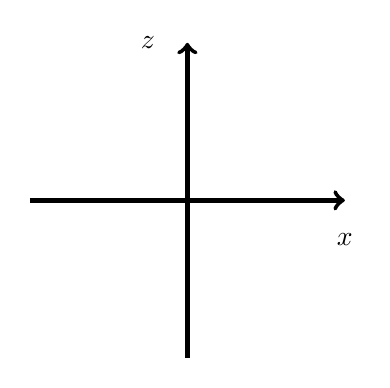
\begin{tikzpicture}
\draw[ultra thick, ->] (-2,0) -- (2,0);
\draw[ultra thick, ->] (0,-2) -- (0,2);
\node at (2,-.5){$x$};
\node at (-.5,2){$z$};
\end{tikzpicture}

\item The traces for $z=0$ and $z=3.$

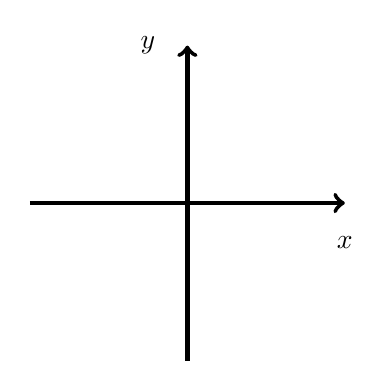
\begin{tikzpicture}
\draw[ultra thick, ->] (-2,0) -- (2,0);
\draw[ultra thick, ->] (0,-2) -- (0,2);
\node at (2,-.5){$x$};
\node at (-.5,2){$y$};
\end{tikzpicture}
\ee
\end{multicols}
\vspace{1in}
\item (2 points) Describe the surface $z=1-x^2.$ Your description can be in words or with a rough sketch. I recommend both.
\vfill
\newpage
\item (4 points) Find any points where the curve $\:\vec{r}(t)=t \: \vec{i} + (2t-t^2) \vec{k}\:$ intersects the paraboloid $\:z=x^2+y^2.\:$
\vfill
\item (5 points) For the curve $\:\vec{r}(t)= \langle \sqrt{t^2+3}, t, \ln(t^2+1) \rangle,\:$ find parametric equations for the tangent line to the curve at the point $\:(2,1,\ln(2)).$ 
\vfill
\item (4 points) Evaluate the integral $\d{\int_0^4 (\: (2t^{3/2}) \vec{i} + \vec{j}+(e^{2t} )\vec{k} \:) dt}$
\vfill
\end{enumerate}
\end{document}